% !TeX spellcheck = <none>
\documentclass[a4paper]{article}
\usepackage{geometry}
\geometry{left=3.5cm,right=3.5cm,top=3.5cm,bottom=3.5cm}
\usepackage{amsmath, amssymb}
\usepackage{graphicx}
\usepackage{subfigure}
\usepackage{pdfpages}
\usepackage{multirow}
\usepackage{float}

\usepackage[citestyle=alphabetic, bibstyle=alphabetic, backend=bibtex]{biblatex}
\addbibresource{ref.bib}

\usepackage{xeCJK}
\setmainfont{Times New Roman}
\setCJKmainfont[BoldFont=SimHei,ItalicFont=KaiTi]{SimSun}

\usepackage{indentfirst}
\setlength{\parindent}{2em}

\usepackage{fancyhdr}
\pagestyle{fancy}
\usepackage{lastpage}
\rhead{}
\lhead{}
\cfoot{\thepage{}}
\renewcommand{\headrulewidth}{0pt}
\renewcommand{\figurename}{图}
\renewcommand{\tablename}{表}
\renewcommand{\abstractname}{摘要}
\renewcommand{\contentsname}{\CJKfamily{SimHei} 目录}

\headheight 14pt

\usepackage{float}

\renewcommand\baselinestretch{1.2}

\begin{document}

%\begin{titlepage}
%\includepdf[pages=2-3,offset=0cm 0cm]{title.pdf}
%\end{titlepage}

\begin{Huge}
	\centering{\textbf{城市表层土壤重金属污染的建模与分析}}
\end{Huge}
\begin{large}
	\begin{flushright}
		
	\end{flushright}
\end{large}
\ \ \\\\

\begin{abstract}
\textit{}
本文主要对于城市重金属污染物的问题进行了研究。我们主要讨论了重金属的分布问题,重金属污染原因分析,重金属传播模型分析以及最终的模型完善以及最后对相关部门提出的一些建议。 \\
\indent 对于重金属分布,我们从平面分布,海拔分布,功能区分布的角度分别对其进行分析。从不同侧面了解到了重金属污染的大致分布状况及分布特点。\\
\indent 而重金属的污染原因分析,我们首先对元素浓度进行了标准化处理,然后建立了因子分析模型。
通过MATLAB,得到前 5 个主因子,然后通过分析重金属元素(主因子)与污染成因(功能区)的相关系数矩阵,
得到造成重金属元素污染的主要原因,最后,利用聚类分析的方法对模型进行了检验,结果表明因子分析模型是基本正确的。\\
\indent 重金属的传播模型的建立,我们类比了热方程对其进行建模。然后又由于重金属污染问题的特殊性,加入了一些修正项。
之后我们用建立的模型对于三种不同的重金属污染治理方案进行数值模拟。
得到了符合实际的结果。并得到了一些对于治理重金属污染比较有效的建议 \\
\indent 第四部分,我们对前面构建的重金属传播模型进行了进一步的完善。加入了土壤降解模型。同时还考虑了水流以及空气对于土壤重金属污染的影响。\\
\indent 最后,根据模型所得结果,从搬迁工业区、增加绿化面积等方面向相关部门提出了治污建议。 

\end{abstract}

\newpage

\tableofcontents

\newpage

\part{引言}
土壤是生态环境的重要组成部分, 也是人类赖以生存的重要自然资源。然而,随着工农业的发展,土壤污染问题越来越突出,尤其是重金属污染,对于土壤的污染尤其严重。
所谓土壤重金属污染是指由于人类的活动将重金属带入土壤中,致使土壤重金属含量明显高于其自然背景值,并造成生态破坏和环境质量恶化的现象。
当前,随着全球经济一体化的发展,我国也加快了工业化与城市化的发展进程,城市的农业集约化程度不断提高。
生产过程中的固体废物不断向土壤表面堆放和倾倒,有害废水不断向土壤中渗透,汽车排放的废气,大气中的有害气体及飘尘不断随雨水降落在土壤中。
这导致水土资源快速恶化和萎缩,土壤利用强度日益加大。   \\
\indent 城市土壤供应着城市绿色植物的生长介质和养分,是城市污染物重要的源和汇,是土壤微生物的栖息地和能量来源,直接影响到城市的生态环境质量。
重金属污染物主要包括汞、镐、铅、铬、锌、铜、镍、钴、锡以及类金属砷等,作为一种持久性有毒物质,进入土壤系统。
从而会使城市土壤的各种性质发生了变化,引起土壤的组成结构和功能发生变化,微生物活动受到抑制,有害物质或分解产物在土壤中逐渐积累,间接被人体吸收,危害人体健康。
因此,土壤重金属污染已成为全球面临的一个严重环境问题。   \\
\indent 国土资源部统计表明,全国320个严重污染区约有548万hm2土壤,大田类农产品污染超标面积占污染区农田面积的20\%,其中重金属污染占80\%,粮食中重金属镉、砷、铬、铅、汞等的超标率占10\%。
在城市,土地污染问题也十分严重。例如,被公认为城市环境质量优良的公园却也存在着严重的土壤重金属污染。
而且我国每年有 1200 万吨粮食遭到重金属污染,直接经济损失超过 200 亿元。
从我国的土地资源情况来看,人均土地资源远远低于世界平均水平,仅及世界人均占有量的1/3。我国耕地人均只有0.1公顷,为世界人均耕地的27.7%。
由此可见,目前我国土地重金属污染非常严重,而且还影响了到人们的食品安全乃至人们的身体健康。
因而如何有效地治理土地重金属污染问题,改良土壤状况,是目前生态环境保护的一个重要主题。    \\
\indent 对于城市而言,土壤的重金属污染治理也十分重要。如果治理不到位,对于城市居民的生命健康会造成巨大的影响。
同时,城市是一个功能极其多样化的地域,粗略地看,城市一般可分为以下 5 类:生活区、工业区、山区、主干道路和公园绿地区,分别记为 1 类区、2 类区、3 类区、4 类区和 5类区。
显然,不同的功能区对于城区而言具有不同的功能,反之,不同的功能区受人类活动影响的程度也不同,重金属的污染程度也不尽相同,治理过程中也应该有所区别。
\indent 现在要求对某一个城区表层的土壤重金属污染进行调查分析。
首先,将所要调查的城区划分成间距为 1 千米的网格状子区域,接着按照每平方公里 1 个采样点的规则,对
表层土壤(大约为 0~10cm 深度)进行采样并编号,然后用 GPS 对采样点定位,记录采样点的位置,包括海拔。
通过专门的仪器测试分析,进一步获得每个样本点所含的多种化学元素的浓度。
此外,还在远离城区和人类活动的地方,按照每两公里 1 个采样点的规则对表层土进行采样,由于人类很少涉足,土壤几乎没有被污染,故可以把其作为城
区表层土壤中化学元素的背景值。\\

\indent 本文以某市不同功能区的表层土壤为研究对象,对土壤中重金属 As、Cd、Cr、
Cu、Hg、Ni、Pb、Zn 的浓度进行测定所获数据进行分析,评价土壤中重金属的污染程度,分析污染的主要原因并定位污染源。
研究过程主要包括以下几个部分:\\
1)给出 8 种主要重金属元素在该城区的空间分布,并分析该城区内不同区域重金属的污染程度。\\
2)通过对数据进行分析,说明造成重金属污染的主要原因。  \\
3)分析重金属污染物的传播特征,并基于此建立数学模型,确定污染源的位置。  \\
4)分析所建立模型的优缺点。为更好地研究城市地质环境的演变模式,确定应该收集的数据信息。基于这些信息,建立一个可以研究地质环境演变模式的模型。  \\

\part{重金属在不同区域的分布情况}
\indent 土壤重金属污染问题成因可能为工业、交通、燃煤、矿区和人类生活等等。在治理过程中,调查清楚某个地区重金属污染的形成原因,对于污染的治理至关重要。
而了解重金属污染的空间分布情况,可以有效的帮助我们判断某个区域污染的缘由。
所以我们首先对重金属的空间分布情况进行研究。这里我们得到了不同重金属的平面分布,海拔分布以及在不同功能区的分布。   \\
\section*{记号表}
\begin{table}[H]
	\centering
	\caption{}
	\label{tab:problem1_symbols}
	\begin{tabular}{ccc}
		\hline
		符号 & 含义  \\
		\hline
		$(x,y,h)$ &取样点的坐标表示   \\
		$C_{ij}$ & 第i个采样点第j种金属的浓度  \\
		$\nu_j$   &  第j种重金属在土壤中含量的平均值  \\
		$\sigma_j$  &   第j种重金属在土壤中含量的标准差 \\
         $\kappa$ & 元素在土壤中的扩散系数      \\
		$\tau$   & 元素在土壤中由地势造成的扩散系数      \\
		$\beta$   &  重金属产生速率            \\
		$\rho(x,y,h,t)$   & 第j种金属在点(x,y,h)时间t时的浓度 \\	
	\end{tabular} \\
\end{table}

\section{重金属的平面分布}
由所给数据中的采样点的x,y坐标以及对应的重金属浓度,我们做出了相应的平面分布图,如下图\ref{fig:char}显示了As以及Pb的污染情况平面图。其中不同颜色表示不同功能区。
圆圈的半径大小与污染程度成正比,即污染越严重,圆圈就越大。
\begin{figure}[h]
	\begin{minipage}[t]{0.5\linewidth}
    \centering
    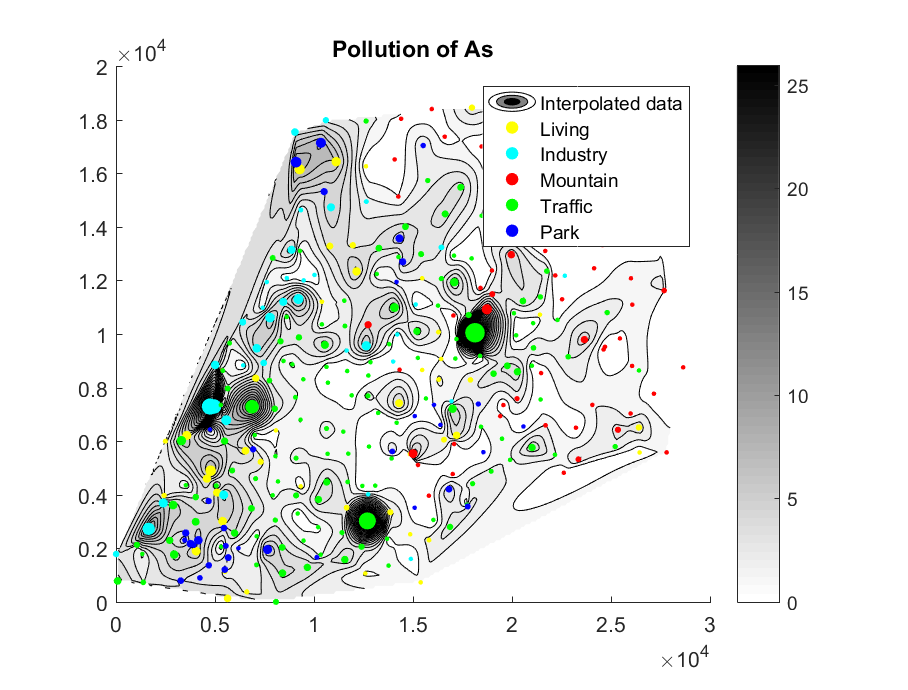
\includegraphics[scale=0.5]{pictures/pollution-of-As.eps}
    \end{minipage}
    \begin{minipage}[t]{0.5\linewidth}
    \centering 
	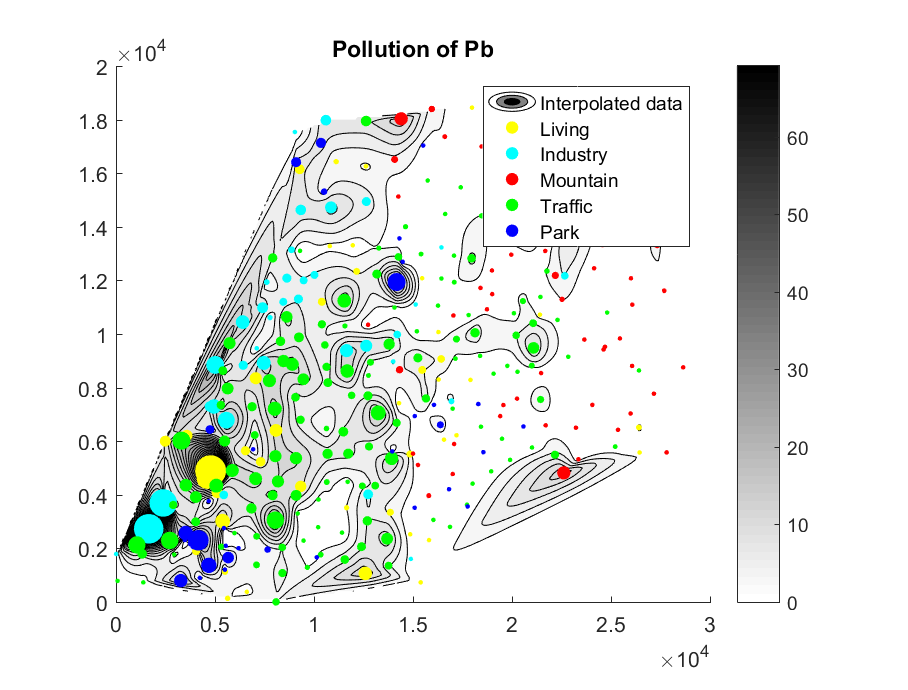
\includegraphics[scale=0.5]{pictures/pollution-of-Pb.eps}
    \end{minipage}
    \label{fig:char}
\end{figure}
从图中能够可以看出:
\indent (1)重金属的分布具有富集性,即重金属在某个区域的分布含量很高,而在其他地方则含量较低。 \\
\indent (2)可以看出As在工业区的分布比较集中,而Pb在交通区域的分布非常密集。                \\
\indent (3)通过对其他重金属元素的平面分布的分析,我们发现不同重金属的分布具有鲜明的特征。往往在某一个区的分布非常密集。 \\
进一步的分析表明:重金属的富集状态实际上是与区域的功能划分息息相关。
比如As主要分布于工业区,这是因为As是一种十分重要化工原料,在工业生产中必不可少,从而在工业区土壤中As含量很高。

\section{重金属的海拔分布}
将海拔每 10 米分一段,假设在某段中共有m个采样点,第i个采样点的重金属j的实测含量为$C_{ij}$,则该段中重金属j的平均含量$W_j$为:
\begin{equation}
W_j=\frac{1}{m}\sum_{i=1}^m C_{ij}
\end{equation}
根据上式,利用采样所得数据分别计算出各种重金属在不同海拔的平均含量。结果如下表所示:
\begin{table}[H]
		\centering
		\caption{不同海拔重金属平均含量}
		\label{average-contend}
		\begin{tabular}{c|cccccccc}
			hight	  &          	As	&   Cd   &     Cr     &   Cu   &     Hg  &    Ni   &     Pb    &   Zn  \\
			\hline
			 0-10m     	&	 7.0714  &  381.23  &  86.288  &  120.46 &   444.88 &   21.147 &   87.784  &  305.11     \\
    			10-20m     	&	 5.8219  &  340.52  &  48.867  &  47.638 &   405.32 &   17.031 &   67.277  &   239.25    \\
   			20-30m    	&	 5.726   &  319.98  &  50.278  &  50.464 &   391.49 &    17.52 &   59.443  &  259.07     \\
    			30-40m     	&	 5.6783  &  316.32  &   57.28  &  54.567 &   645.86 &   16.609 &    67.79  &  164.09     \\
    			40-50m     	&	 6.6211  &  328.15  &  42.978  &  39.453 &   117.18 &   16.979 &    52.31  &  154.99     \\
    			50-60m      	&	 5.125   & 260.62   & 41.036   & 43.522  &   66.08  &  14.783  &  55.222   & 124.81      \\
    			60-70m     	&	 4.4469  &  190.19  &  38.328  &  21.978 &   33.826 &   13.102 &   39.961  &   101.6     \\
    			70-80m     	&	 4.7492  &  264.49  &  55.809  &  30.905 &   60.671 &   22.693 &   9.755  &  205.65     \\
    			80-90m     	&	 3.8433  &  129.42  &  37.658  &  15.522 &   45.657 &   15.437 &   36.007  &  72.842     \\
    			90-100m    	&	 4.686   & 180.75   & 31.781   & 16.278  &  24.822  &  12.979  &  32.405   & 71.958      \\
    			>=100m    	&	 3.3381  &  168.67  &  34.459  &  12.831 &   37.124 &   13.316 &   38.689  &  73.364     \\
		\end{tabular}
	\end{table}
由上面的数据可以看出,
\begin{itemize}
\item 总的来说各种重金属元素的含量随着海拔的升高而降低。这可能是因为人类活动的区域主要在低海拔地区,高海拔区受人类的影响较小。
\item 但是可以大致的看出不同的重金属含量随海拔的变化率是有区别的。有些金属的随海拔变化的十分剧烈
\item 此外,还可以发现,在70~80m的海拔高度上,大部分的重金属元素含量都要高于附近的海拔高度地区。
这一海拔高度多为山区,重金属含量高可能是因为汽车尾气,工厂废气中所含的重金属随大气运动进入这一地区的土壤所致。
也有可能是因为这一地区有采矿场的缘故。

\end{itemize}
从数据可以看出,不同的重金属元素的含量有很大的差别。
为了排除不同金属元素原本在土壤中含量差异的影响,我们对不同金属做了标准化处理:
\begin{equation}
W_j^{\prime} = \frac{W_j - \nu_j}{\sigma_j}
\end{equation}•
经过处理之后的数据变为:
\begin{table}[H]
		\centering
		\caption{不同海拔重金属相对平均含量}
		\label{average-contend}
		\begin{tabular}{c|cccccccc}
			hight	  &          	As	&   Cd   &     Cr     &   Cu   &     Hg  &    Ni   &     Pb    &   Zn  \\
			\hline
			 0-10m     	&	 3.9002  &   8.4187   &  6.2023  &  29.858  &   51.399  &   2.3893  &   9.5012  &   16.927    \\
    			10-20m     	&	 2.5713  &   7.1518   &   2.072  &  9.6047  &   46.612  &   1.3548  &   6.1152  &    12.28    \\
   			20-30m    	&	 2.5378  &   6.4723   &  2.2459  &  10.381  &   45.157  &   1.5129  &   4.8493  &   13.713    \\
    			30-40m     	&	 2.3626  &   6.3342   &  2.9309  &  11.491  &   76.801  &   1.1732  &   6.2091  &   6.9488    \\
    			40-50m     	&	 3.3905  &   6.8669   &  1.3438  &  7.2926  &   10.683  &   1.2863  &   3.6197  &   6.3921    \\
    			50-60m      	&	 2.0105  &   4.5835   &  1.3605  &  8.5117  &   4.6513  &   1.0349  &    4.149  &   4.2198    \\
    			60-70m     	&	 1.2583  &   2.3302   &  1.0627  &   2.576  &   0.7807  &  0.57632  &    1.779  &   2.6758    \\
    			70-80m     	&	 1.7538  &   4.9559   &  2.9497  &  5.0481  &   3.7748  &   2.9664  &   5.1249  &   9.9593    \\
    			80-90m     	&	 0.66852 &   0.63333  &  0.87556 &   1.1023 &    1.6667 &   0.95439 &    1.0514 &     1.071   \\
    			90-100m    	&	 1.5422  &    2.169   & 0.59156  &  1.0714  &  0.11075  &  0.64079  &  0.72533  &    0.902    \\
    			>=100m    	&	 0.2679  &   1.7252   & 0.89564  &  0.4606  &  0.85681  &  0.75185  &   1.5467  &  0.81016    \\
		\end{tabular}
	\end{table}
对于处理之后的数据,我们还发现:
\begin{itemize}
\item 可以看出,大部分的低海拔地区的相对平均含量都超过了3,有些甚至有50。而根据正态分布的原理可知,观测值在3倍标准差以外的概率已经是非常小了。
从而我们推断,该城市的土壤污染状况不容乐观,应该立即采取措施进行治理。
\item Cu和Hg随海拔高度的变化比较剧烈,这也验证了标准化之前观察的现象。这说明海拔较低地区的Cu和Hg的污染比较严重,在治理过程中应该加大力度。
\end{itemize}
\section{不同区域重金属污染情况}
对于不同区域,我们假设某区域有m个数据点,则该区域的重金属j的平均含量$W_j$为:
\begin{equation}
W_j=\frac{1}{m}\sum_{i=1}^m C_{ij}
\end{equation}
\indent 同样的,我们也对其进行标准化,最终的得到的结果如下:
\begin{table}[H]
		\centering
		\caption{不同功能区重金属相对平均含量}
		\label{average-contend}
		\begin{tabular}{c|ccccc}
			hight	  &    Living  &  Industry  &  Mountain  &  Traffic  &   Park    \\
			\hline
			As   & 3.0475  &  4.1849   &   0.94613   &  2.4705   &   3.0165      \\
    			Cd   & 5.4836  &  8.7963   &    1.3074   &  7.7873   &    5.145		\\
    			Cr   & 4.2767  &  2.6107   &    1.2889   &  3.0671   &   1.4916		\\
    			Cu   & 9.3057  &  31.764   &    1.5308   &  13.618   &   4.7729		\\
    			Hg   & 7.7496  &  76.198   &    1.4151   &  51.909   &   10.504		\\
    			Ni   & 1.6847  &  2.0983   &    1.2222   &  1.5027   &  0.93707		\\
    			Pb   & 6.4211  &   10.34   &    1.3029   &  5.5056   &   4.9816		\\
    			Zn   & 12.133  &  14.949   &   0.86168   &   12.53   &   6.3503		\\
		\end{tabular}
	\end{table}
由表中数据可知: 
\begin{itemize}
\item 工业区和交通区的各种重金属污染均比其他区域的要严重。比如工业区的Hg含量大约是生活区Hg含量的10倍多。                               
\item 山区的各种重金属的含量均比其他区域要小。通过对比可以说明,该城市的土壤污染是由于人类的活动造成的,而不是由于原本的土壤质量就很差。  
\item 对于金属As和Pb,可以看出As和Pb在工业区的含量最高。这可能是因为As和Pb都是重要的化工原料,许多工厂的废渣,废水,废气中都含有As和Pb,从而导致工业区周围As和Pb含量较高。
\item 对于金属Cu和Hg,它们在生活区,工业区以及交通区的含量都比较高。
尤其是Hg,在工业区和交通区的含量非常之高,污染非常的严重。Cu和Hg也是十分重要的化工元素,在工业区含量较高也十分正常。
同时照明用灯,煤炭中均含有Hg元素,从而照明用灯的随意丢弃,大量煤炭的燃烧都会使得环境中的Hg含量大大上升,同时汽车尾气中也含有Hg以及Cu。
在这些因素的作用下,使得这几个功能区的Cu和Hg的含量量较高。
\end{itemize}


\part{重金属污染原因分析}
通过前面的分析,可以知道土壤重金属污染主要是由于人类活动而引起的。
这一部分,我们将仔细的分析造成这些污染的具体成因。
粗略的来说,这些重金属污染主要与工业生产、人类生活以及交通运输有关。
工业生产中的废水废气中的重金属经过一段时期,就会进入土壤中得到富集。
日常生活中的各种垃圾,比如废旧电池,废旧电子线路板等等,其中有些重金属的含量非常高,不经过处理就直接投放的环境中,将会对周围的土壤造成很大的污染。
而交通运输中产生的汽车尾气中也会含有重金属,比如Pb、Cu等金属元素。在第二部分中对不同的重金属分布数据中也能看出这些元素在交通区的含量都非常高。
此外,同一种重金属的产生也可以来自多个方面。               \\
比如土壤中Hg的来源,可以来自矿物燃料燃烧排放;电气、仪表、氯碱、涂料等许多企业生产中要消耗大量汞和汞化合物;同时以前还有含汞农药的广泛使用,也造成了土壤汞的污染。
\indent 因此为了更好的鉴别该地区土壤重金属污染的成因,我们采用统计分析中的因子分析方法对8种重金属的可能污染原因进行统计分析。
\section{数据的预处理}
\subsection{重金属浓度的标准化}
\indent 由于采样点不同重金属的浓度单位不同,而且不同重金属的含量差异较大。
所以我们需要将不同重金属的含量标准化,来排除上述原因造成的影响,以方便后面对于不同重金属污染形成原因的分析。第i个观测点的第j重金属的含量$C_{ij}$标准化为:
\begin{equation}
C_{ij}^{\prime}=\frac{C_{ij}-\nu_{j}}{\sigma_{j}}
\end{equation}
根据以上公式,我们就可以得到标准化后的数据。
\subsection{特征块的构造}
构造一个区域$S_{all}$,使得整个城区在该区域中。
取$S_{all}=30000*20000m^2$。根据城区的功能分布,功能区一共有5种,记为$f_i$,$i=1,2,3,4,5$,分别代表生活区、工业区、山区、交通区和公园绿地区。
对于属于上述5种功能区的采样点,我们称其为有效点。对于不在该城区的点,我们称其为无效点。\\
\indent 对于整个区域的采样点按照功能区的不同进行计数,记为$n_k$($i=1,2,3,4,5$)。则总的有效点数为:
\begin{equation}
n=n_1+n_2+n_3+n_4+n_5
\end{equation}
\indent 定义$p_k$($i=1,2,3,4,5$)分别表示区域内分属于生活区、交通区、公园绿地区、山区和工业区的有效点的个数占每个区域内总有效点的比率,即:
\begin{equation}
p_k=\frac{n_k}{n}
\end{equation}
不同的功能区会造成不同的重金属污染,产生的重金属的多少也不相同。在该模型中我们用$p_k$表示各个功能区在
区域中对重金属污染做出的“贡献”大小,即每个功能区产生的污染与总污染量之比。
\section{因子分析模型的建立}
因子分析法是一种从研究的大量变量之中找到独立的潜在变量的一种方法。目的在于对原来的高维变量进行降维。
将每一个原始变量分成两部分,一部分是少数几个公共因子的线性组合,而另一部分是该变量所独有的特殊因子。 \\
\indent 设 p 维总体$x=(x_1,x_2,\cdots,x_p)$的均值为$\nu=(\nu_1,\nu_2,\cdots,\nu_p)$,协方差矩阵为$\Sigma=(\sigma_{ij})_{p*p}$,相关系数矩阵为$R=(\rho_{ij})_{p*p}$。
则因子分析的一般模型为:
\begin{equation}
\left\{
\begin{aligned}
x_1=\nu_1+a_{11}F_1+a_{12}F_2+\dots+a_{1m}F_m+\epsilon_1    \\
x_2=\nu_2+a_{21}F_1+a_{22}F_2+\dots+a_{2m}F_m+\epsilon_2    \\
\vdots
x_p=\nu_p+a_{p1}F_1+a_{p2}F_2+\dots+a_{pm}F_m+\epsilon_p    \\
\end{aligned}
\right.
\end{equation}
其中$F_1,F_2,\cdots,F_m$为m个公共因子,$\epsilon_i$是$x_i(i=1,2,\cdots,p)$所独有的特殊因子。这些都是不可观测的潜在变量。
写成矩形式,即为:
\begin{equation}
x=\nu+AF+\epsilon
\end{equation}
其中$A=(a_{ij})_{p*m}$称为因子载荷矩阵,$F=(F_1,F_2,\cdots,F_m)$称为公共因子向量,$\epsilon=(\epsilon_1,\epsilon_2,\cdots,\epsilon_p)$称为特殊因子向量。
\subsection{模型的求解}
对于因子分析方法,关键在于确定因子载荷矩阵以及最优的公共因子的个数。我们先来考虑因子载荷矩阵的计算。这里我们采用主成分的方法来进行计算。\\
由谱分解理论我们知道,协方差矩阵$\Sigma$有如下分解式:
\begin{equation}
\begin{aligned}
\Sigma &=\lambda_{1} e_{1} e_{1}^{\prime}+\lambda_{2} e_{2} e_{2}^{\prime}+\cdots+\lambda_{p} e_{p} e_{p}^{\prime}  \\
       &=\left(  
      \begin{array}{cccc}  
          \sqrt{\lambda_1}e_1 & \sqrt{\lambda_1}e_1&\cdots&\sqrt{\lambda_p}e_p
  \end{array}  
  \right)  
  \left(  
  \begin{array}{c}  
           \sqrt{\lambda_1}e_1^{\prime} \\  
          \sqrt{\lambda_2}e_2^{\prime}\\  
         \vdots                      \\
         \sqrt{\lambda_p}e_p^{\prime} \\
 \end{array}  
 \right)  
\end{aligned}
\end{equation}
其中$\lambda_1 \geq \lambda_2 \geq \cdots \geq \lambda_1 \geq 0$为$\Sigma$的特征值,$e_1,e_2,\cdots,e_p$为其特征向量,$e_i^{\prime}$为$e_i$的转置。
此时公式(9)中的因子分析是精确的。但是它并没有达到降低维数的目的。因此,当后p-m个特征值较小时,我们就略去这p-m个向量对于公式(9)的贡献。从而得到近似:
\begin{equation}
\begin{aligned}
\Sigma & \approx \left(  
      \begin{array}{cccc}  
          \sqrt{\lambda_1}e_1 & \sqrt{\lambda_1}e_1&\cdots&\sqrt{\lambda_m}e_m
  \end{array}  
  \right)  
  \left(  
  \begin{array}{c}  
           \sqrt{\lambda_1}e_1^{\prime} \\  
          \sqrt{\lambda_2}e_2^{\prime}\\  
         \vdots                      \\
         \sqrt{\lambda_m}e_m^{\prime} \\
 \end{array}  
 \right)  
   & =AF
 \end{aligned}
\end{equation}
从而我们就得到了因子荷载矩阵。\\
对于公共因子的数量选择,我们通过MATLAB进行数值模拟,从中选择出最为合适的数目。
\subsection{因子旋转}
用上面的方法虽然得到了因子载荷矩阵,但是其结构往往比较复杂,往往一个变量会受到几个公共变量的影响。这并不是我们所乐于看到的。
我们希望找到一种的载荷模式,它使得各变量在某单个因子上有高额载荷,而在其余因子上只有娇小的载荷。
为了解决这个问题,我们可以对因子进行旋转,即:
\begin{equation}
\hat L^* = \hat LT
\end{equation}
其中$TT^{\prime}=I$,即$T$为正交矩阵。
这样,我们就能够找到比较好的公共因子。
\section{重金属元素因子分析}
对于这个复杂的问题,我们做如下假设:\\
简化性假设:造成重金属污染的主要原因只考虑工业、交通、燃煤、矿区和人类生
活。\\
概括性假设:因子分析中累计贡献率超过 85\%即认为是涵盖了源数据的全部信息量. \\
惟一性假设:每一种重金属元素属于且仅属于一个因子。\\
\indent 有了上面的假设,我们就可以来进行重金属元素的因子分析了。
由于同一种活动可以产生多种重金属元素,即不同种类的重金属元素之间可能彼此相关,故首先对 8 种重金属污染物进行因子分析,从中发现不同重金属元素之间的相互关系。
我们对于数据经过上面的处理,当因子数取为5时,因子的累计贡献率超过85\%。所以我们将因子数确定为5。
得到因子载荷矩阵后,我们又做了因子旋转使得因子载荷矩阵的结构尽量的简单,得到如下结果:
\begin{table}[H]
		\centering
		\caption{}
		\label{average-contend}
		\begin{tabular}{c|ccccc}
			元素	  &   f1   &  f2  &   f3 &   f4  &   f5   \\
			\hline
			 As   &  0.024061 &   -0.017133  &    0.98028  &  -0.0036262  &  -0.013104    \\
    			 Cd   &   0.73828 &   0.0089358  &  -0.005822  &   -0.048483  &  -0.051178    \\  
    			 Cr   &  0.037436 &    -0.65547  &  -0.090772  &   -0.037973  &  -0.012617    \\
    			 Cu   &   0.12187 &    -0.37687  &  -0.095855  &     0.44761  &   -0.12449    \\
   			 Hg   &  -0.05934 &      0.1544  &   0.048142  &     0.89044  &   0.060712    \\
   			 Ni   & -0.099508 &    -0.63489  &    0.13686  &  -0.0089397  &    0.06049    \\
   			 Pb   &   0.65125 &    0.016763  &   0.019314  &    0.053432  &   0.061484    \\
   			 Zn   &  0.023677 &   -0.027363  &  -0.013115  &  -0.0041498  &     0.9851    \\
		\end{tabular}
\end{table}
变量与某一个因子的联系系数$a_{ij}$绝对值(载荷)越大,则该因子与变量关系越近。
经分析可知,
\begin{itemize}
\item Cd和Pb元素与$F_1$的载荷系数都比较大,分别为0.73和0.65,均在各自的五个载荷系数中,占据了主导地位。所以可以认为因子$F_1$可以理解为Cd与Pb的组合。
\item 而Cr和Ni的$F_2$载荷系数为-0.65和-0.63,占据了较大比例。所以我们把$F_2$看成Cr与Ni的组合。另外,值得注意的是Cu的载荷系数为-0.37,也比较大。
\item 因子$F_3$对于As的载荷系数为0.98,与As的相关性非常高,所以$F_4$可以单独看成是As元素的影响。
\item 对于因子$F_4$,Hg的载荷因子为0.89,与其他重金属相比最大。另外Cu的载荷因子为0.44,居于第二。
这里要注意Cu元素,根据数据,它的$F_2$以及$F_4$的荷载系数都比较显著,对于Cu应该属于$F_2$还是$F_4$,还应该有更深入的讨论。
但在这里由于我们假设每种金属元素只属于一个因子,所以这里我们暂时认为$F_4$为Cu的因子。
\item 对于Zn元素,可以明显的看出因子$F_5$的载荷系数为0.98,对于Zn的含量有着决定性的影响。所以我们认为因子$F_5$代表Zn元素的影响。
\end{itemize}
通过上述因子分析我们已经确定:
\begin{itemize}
\item 因子1包含了 Cd 和 Pb 元素,由相关系数矩阵可知,因子1与交通区的相关度最大,所以我们可以判断因子1污染的原因的交通。
再从因子浓度分布图中得到,因子1 浓度较高的地带分布比较广泛,与交通区遍布大部分城区的情况相吻合,又与汽车尾气中含有较多
的 Cd 和 Pb 元素这一事实相结合,可以确定因子1污染的原因是汽车尾气,属于交通污染。  
\item 因子2主要是 Cr 和 Ni 的组合,外加部分 Cu。 
由相关系数矩阵可知,因子2与交通区最相关,同时与生活区和工业区也有一定的相关度。 
由图可知,因子2在该城区的大部分区域浓度都是很低的,主要富集在该城区图的左下角。
综上所述我们可以得出因子2污染来源于某种工厂。由于 Cr 的污染主要来源于金属加工、电镀、制革、
冶金、水泥等工业,Ni 污染的主要来源是不锈钢和抗腐蚀合金,以及镀镍、铸币行业,Cu 污
染的原因在于铜锌矿的开采和冶炼、金属加工、机械制造、钢铁生产等,
由此我们可以推断,因子2污染的主要原因是在城区的左下角有从事金属加工钢铁生产的工厂,属于工业污染。
\item 因子3为元素 As,由相关系数矩阵可知,As 的浓度主要与生活区和工业区相关。
从图中亦可看出,As 主要分布在工业区和生活区比较密集的地方。
在工业区附近,As 污染主要是经各种工业生产产生,在生活区附近,则有可能是砷农药的使用导致了砷污染,
同时,工业区和生活区都可能经煤燃产生 As 污染。所以,因子3,即 As 污染的原因是工业污染、燃煤污染和生活污染。    
\item 因子4为元素 Hg,外加部分的 Cu,由相关系数矩阵可知,Hg 的浓度与山区和交通区相关性较大,与生活区也有一定的相关性。
再由因子浓度分布图可得,Hg 主要分布在临近生活区和工业区的区域。
可以断定,Hg 的污染主要是由于燃煤造成的,无论是工业用煤还是居民用煤,都会造成地表土受到 Hg 的污染。
而且,Hg 的浓度与交通区相关,Hg 又大量存在于汽车尾气当中,所以 Hg 污染也属于交通污染。
此外,Hg 的浓度也与山区相关,很可能是由于某山区上存在汞矿。
所以,因子4,即 Hg 污染的原因既有燃煤污染,亦有交通污染,也可能有矿区污染。    
\item 因子5是元素 Zn。由相关系数矩阵可知,Zn 元素的浓度与生活区、工业区和交通区十分相关。
再可以通过图看出,一部分 Zn 分布在工业区,另一些则分布地较无规律。
由于 Zn元素的主要污染源有冶炼加工、机械制造以及镀锌等工业的排放,可以断定,分布在工业区的 Zn 污染属于工业污染。
此外,考虑到无规律分布的 Zn 的污染,可能是锌矿的开采导致的。所以,Zn 元素的污染原因既是工业污染,又可能是矿区污染。
\end{itemize}
\indent 从而根据上述分析,我们可以得出8种重金属的不同的产生原因,结果如下表:
\begin{table}[H]
		\centering
		\caption{重金属污染的主要原因表}
		\label{main-reason}
		\begin{tabular}{|c|c|}
		\hline
			重金属元素	  &  造成污染的主要原因 \\
			\hline
			Cd,Pb  &    交通污染  \\  \hline
			Cr,Ni,Cu  &    工业污染 \\ \hline
			Hg,Cu   &   燃煤污染,交通污染,矿区污染 \\ \hline
			As   &	工业污染,燃煤污染,生活污染  \\ \hline
			Zn  &     工业污染,矿区污染        \\ \hline
		\end{tabular}
\end{table}
\section{模型的聚类分析}
为了进一步验证因子分析的合理性,可以使用聚类分析来验证因子分析的结果。
聚类分析是通过使用一种相似性度量来比较不同数据之间的距离,并将距离相近的数据归为一类,最终将数据划分成几类的分析方法。
我们这里使用MATLAB中的clusterdata函数来做聚类分析。
我们对 8 重金属元素进行聚类分析,得到如图\ref{fig:cluster}的系统树:
\begin{figure}
    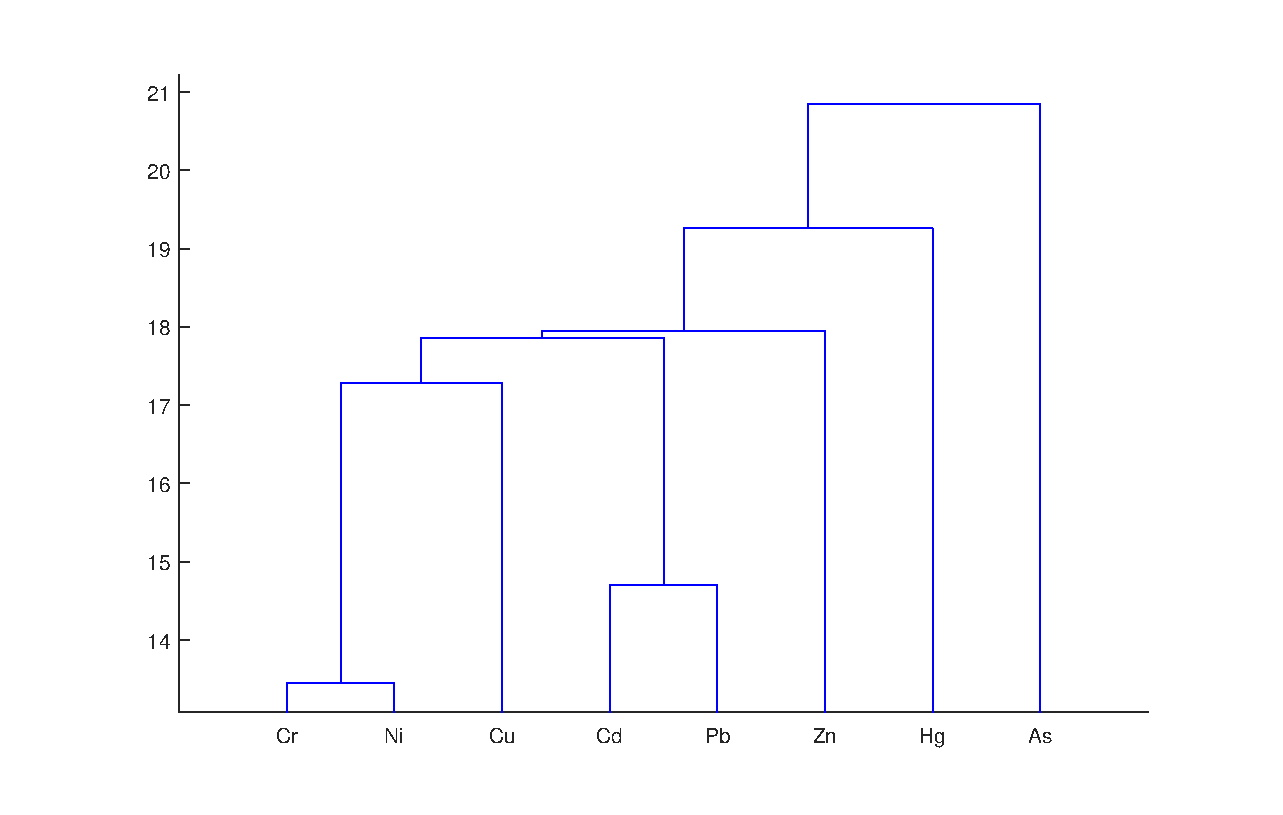
\includegraphics[width=0.6\textwidth,bb=80 420 500 720]{pictures/cluster.eps}
    \caption{8种重金属聚类分析结果}
    \label{fig:cluster}
\end{figure}
由上图可知, 根据因子分析所确定的主因子数为 5,故将这 8 种重金属元素聚成 5 类。
在系统聚类树上容易看出,Cr和Ni元素为一类,Cd 和Pb元素为一类,其余元素皆是自成一类。
由于要分成5类,所以,我们把Cr,Ni和Cu合成一类。
在上面的因子分析中,Cu与$F_2$和$F_4$的载荷系数均比较显著,我们最后将其归于$F_4$中。而通过聚类分析,我们得出,将Cu与Cr和Ni归为一类更为合理。
还可以看到的是,Zn 与包含 Cd 和 Pb 的一类元素相距很近,即相似度较高,说明Zn和Pb相对而言还是较为相似的。
由此可以看到,聚类分析的结果与前面因子分析的分类结果基本一致,因子分析的结果是比较合理且可靠的。


\part{重金属污染物传播模型}
上一节中,我们通过因子分析以及聚类分析,分析出了8种重金属污染物的产生原因。
在这一部分,我们将先找到污染源的位置,再对于重金属产生后的传播过程进行建模分析,并提出不同的方案,比较不同方案对污染的治理效果。\\
\indent 传播特征理解为不同重金属污染物在空间上的不同分布模式。
这种相对稳定的空间分布模式是由于重金属元素随着时间的推移而不断扩散的结果,故能够反映重金属污染物的传播特征。
首先,我们通过建立各向同性介质下的重金属污染物扩散偏微分方程。
\section{重度污染区分析}
当我们获得城市土壤重金属污染数据后,我们首先需要找到污染源的具体位置。\\
\indent 为了解决这个问题,我们首先要对离散的数据进行网格化处理。我们用插值的方法利用这些离散的数据点去估算格点的数值。
在插值时,我们使用德劳内三角化来进行计算。
这里我们使用了MATLAB中的\emph{scatteredInterpolant()} \cite{journals/jei/Amidror02}对已有的数据进行插值算法,求出网格上的点的近似值。
% todo: algorithm
\subsection{污染源的确定}
对于污染源,我们认为其重金属排放速率是局部最大的。
而且,一般来说,污染源附近的重金属含量是要高于周围的区域。
因此,为了找到污染源,我们可先通过重金属的含量找到存在污染源的可疑区域。
所以我们选择一个适当的半径b,找到所有这样的格点,使其在以半径为b的邻域内重金属的含量为最大值,即
\begin{equation}
\rho_{ij} \geq \rho_{i+k, j+l}, for\ \forall \ |k|, |l| \le b
\end{equation}
通过上述方法,我们就可以从该区域中找到重金属含量较高的极大值点,也就是污染源疑似点。
为了从中确定真正的污染源,我们需要引入重金属传播速率$\beta$来描述不同点的向周围传播重金属的速率。\\
\indent 我们假设重金属的含量分布服从高斯分布。
从而对于每一个污染源,它的污染传播速率会正比于该污染源的重金属含量,也即:
\begin{equation}
\beta \propto \rho^2
\end{equation}
我们认为,污染源具有最大的污染传播速率$\beta$,所以我们对得到的重金属含量极大值点,分别求出这些点的重金属传播速率,将其中的重金属传播速率在前50\%的点作为污染源。
经过模拟,我们分别找到了因子$F_1,\cdots,F_5$的污染源分布。
图\ref{fig:polluted-source}为因子$F_5$的污染源分布图。
\begin{figure}
    \centering 
    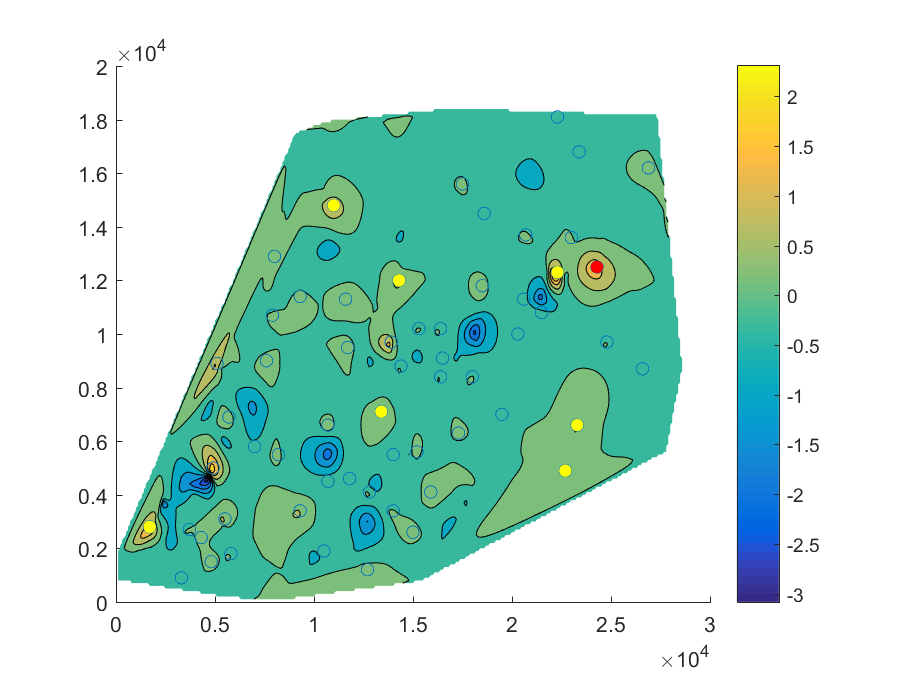
\includegraphics[scale=0.9]{pictures/polluted-source.eps}
    % todo: which index
    \caption{因子$F_5$污染源分布图}
    \label{fig:polluted-source}
\end{figure}
图中用黄色和红色点标出的即为污染源,其中红色点表示污染最为严重的点。
可以看出,图中一共有8个污染源,主要分布在工业区和山区,这与我们前面所分析的$F_5$的主要原因为工业污染和矿区污染相符合。
这说明我们寻找污染源的方案还是十分可靠的。
\subsection{与掩膜法的比较}
在一些文献 \cite{GEAN:GEAN338} \cite{mitchell_2012} 中提到了所谓的“掩膜法”,可以理解成是一种带窗口的空间傅里叶变换。
在这里我们并没有使用这一种方法,是在比较权衡后考虑了两种方法各自的优劣。

掩膜法能够非常好地估计每一个点的附近的污染程度;
但是比较大的问题在于在使用卷积获得该空间频率的能量之后,无法立即指出能量分布集中的位置。
另一方面,掩膜法是否能细化污染源与周边点的浓度差异依赖于对于“膜”形状参数的选取;而这一点通常不是容易的。

前文所使用的方法中,虽然看似比较直接,但是由于在污染局部附近总是由局部最大值的存在(这依赖于搜索范围有界这一事实),我们能够迅速给出局部能量集中的位置。
为了衡量不同污染源排放的程度,我们试图使用正态分布来近似估计每个污染源周边的情况,但是结果却与数据相去甚远。
经过分析我们认为污染源浓度是一个更为主要的因素,因此最后将浓度的平方作为衡量污染情况的指标。

值得注意的是,掩膜法与前文所使用的方法并不是完全互斥的。
实际上掩膜法在进行筛选的时候仍然要考察相邻点的差异性,而本文所使用的方法其实也是平衡了数据偶然的波动性。

\subsection{重金属传播的基本微分方程}
确定了重金属的污染源之后,我们要对重金属的扩散过程进行建模,这样我们才能对于城市土壤的变化趋势作出预测。  \\
\indent 对于重金属的扩散,我们先考虑最为简单的情形。
各向同性介质下的重金属传播算是最为简单的情形,例如重金属在平原均匀土壤中的渗透和重金属在无风空气中的扩散均属于此种情况。
在这种情况下,我们可以把中心的污染源看成是一个热源,从而重金属的传播过程就可以看做是热源传热的过程。
从而我们得到这种情况下,重金属的扩散近似的满足热方程:
\begin{equation}
\frac{\partial \rho}{\partial t} = \kappa \Delta \rho
\end{equation}
由于我们主要考虑的是土壤表层的重金属污染分布,所以上式实际上化为一个二元偏微分方程。
我们以污染源为极点,将上述方程变换到极坐标系,得:
% todo: remove
\begin{equation}
\frac{\partial \rho}{\partial t} = \kappa(\frac{\partial^2 \rho}{\partial r^2}+\frac{1}{r}\frac{\partial \rho}{\partial r})
\end{equation}
当扩散过程达到稳态时,有$\frac{\partial \rho}{\partial t} = 0$,此时可以求出解析解为:
\begin{equation}
\rho(r) = \frac{Q}{r}
\end{equation}
其中$Q$为待定常数。\\

\indent 而对于一般情况,我们不仅要考虑上面的“热扩散”过程,还要把由地势造成的对扩散速率的影响考虑在内。
地势对于重金属的扩散造成的影响,其实是在重力作用下,重金属向低处的扩散速率会大于向高处的扩散速率。
在这里,我们认为由于地势对于扩散速率造成的影响与地势的二阶偏导成正比。实际的扩散速率是热扩散速率与地势造成的影响之差。
从而我们得到如下重金属扩散应当满足的方程:
\begin{equation}
\frac{\partial \rho}{\partial t} 
= (\kappa_x\frac{\partial^2 \rho}{\partial x^2}+\kappa_y\frac{\partial^2 \rho}{\partial y^2}+\kappa_z\frac{\partial^2 \rho}{\partial z^2})
+( \tau_x\frac{\partial^2 \rho}{\partial x^2}+\tau_y\frac{\partial^2 \rho}{\partial y^2}+\tau_z\frac{\partial^2 \rho}{\partial z^2})*\rho
\end{equation}
写成向量形式,即为:
% todo: fix formula
\begin{equation}
\frac{\partial \rho}{\partial t} = \kappa \Delta \rho + \tau \Delta h *\rho
\end{equation}
上面的模型都是对于污染源不在产生新的重金属而言的。而对于不断产生新污染的情形,则我们还要再加上一个修正项重金属产生速率$\beta$,所以对于污染源,原方程修正为:
\begin{equation}
\label{eqn_model}
\frac{\partial \rho}{\partial t} = \kappa \Delta \rho + \tau \Delta h *\rho + \beta
\end{equation}
这就是我们得到的重金属传播过程所满足的偏微分方程。  \\
\indent 这里要注意的是,上面的分析是对于连续变量的分析。
对于我们所测得的离散数据,我们去要对上述公式做离散化处理。
对于$\delta \rho $,在离散的数据中,我们用数据的二阶差分来表示它,即:
\begin{equation}
\Delta \rho= \rho_{i+1}+\rho{i-1}-2\rho_i
\end{equation}
在下面的数值模拟过程中,通过具体的数据,我们也会比较我们所加的修正项对于最终传播结果造成的影响。


\section{城市未来地质环境预测}
有了前面的工作,我们就可以通过模拟来预测不同的污染源治理方案对于未来的城市土壤环境的造成的影响。
通过分析不同的治理方案造成的影响,我们比较了不同方案的利弊,从而为重金属污染的治理提出一些合理的建议。

\subsection{去除污染源后的城市土壤变化}
这里我们假设城市对于污染源的处理十分彻底,将产生污染的各种源头统统控制住。
也就是说,经过治理,原先的污染源不在产生新的重金属。此时,原本在污染源附近的重金属含量较高的地区仍然会向周围扩散。
此时我们先考虑这些重金属的扩散为各向同性传播。此时污染的传播方程比较简单:
\begin{equation}
\frac{\partial \rho}{\partial t} = \kappa  \Delta \rho\kappa  
\end{equation}

在模拟时,我们将$\kappa$设为0.2,这样我们就可以得到土壤中重金属含量随时间的变化图像。
\subsection{维持污染源的城市土壤变化}
为了进行对比,我们假设所有的污染源依然不断地产生重金属污染,从而可以看出消除污染源之后对于该城区土壤重金属含量的影响。
对于不是污染源的地区,其满足的微分方程与上一小节的方程相同。
而对于污染源所在的地点,我们们还必须加上其产生重金属污染物的速率$\beta$。所以在污染源地区,需满足:
\begin{equation}
 \frac{\partial \rho}{\partial t}= \Delta \rho * \kappa + \beta
\end{equation}
作为估计,我们将$\beta$设为0.03,这是由于在上面确定污染源时,计算得出的污染源的重金属产生速率大致在0.03附近。
我们以观测数据为起点,模拟了该城区一年的
\subsection{考虑高度影响的城市土壤变化}
城市的地形高度并不是一成不变的,事实上,城市的地形其实十分复杂。下面是该城区的地形示意图:
\begin{figure}
    \centering 
    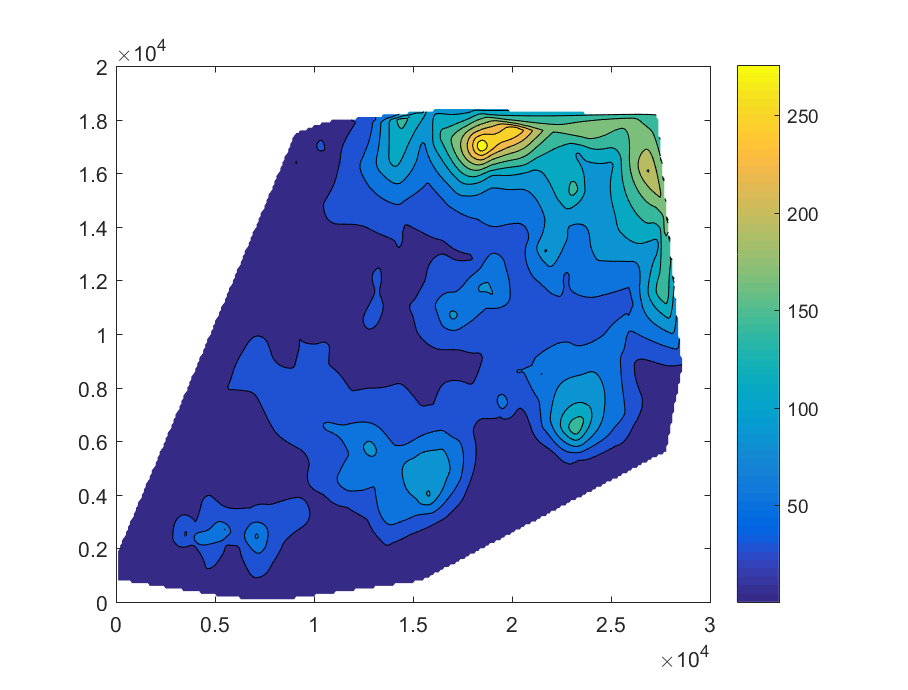
\includegraphics[scale=0.8]{pictures/height.eps}
    \caption{城市地形示意图}
    \label{fig:height}
\end{figure}
当我们考虑到城市的地形对于重金属污染的影响时,根据前面的讨论,我们需要加上地势造成影响的修正项,即:
\begin{equation}
 \frac{\partial \rho}{\partial t}= \Delta \rho * \kappa + \Delta h * \tau * \rho + \beta
\end{equation}
我们认为,由地势造成的扩散系数较小,为0.002,$\kappa$的大小与前面保持相同,仍为0.2。

在模拟中,我们选择对金属Cd进行模拟,这是因为Cd的污染源分布既有比较分散的污染源,还有相对集中的污染源。
这样对于Cd进行模拟,我们既能够看出每个污染源对于其周围的土壤产生的影响,还能够观察到不同污染源相互作用后对土壤造成的污染。
经过模拟,我们得到如图\ref{fig:pollution-with-hight}所示的结果:
\begin{figure}
    %\centering 
    \flushleft
    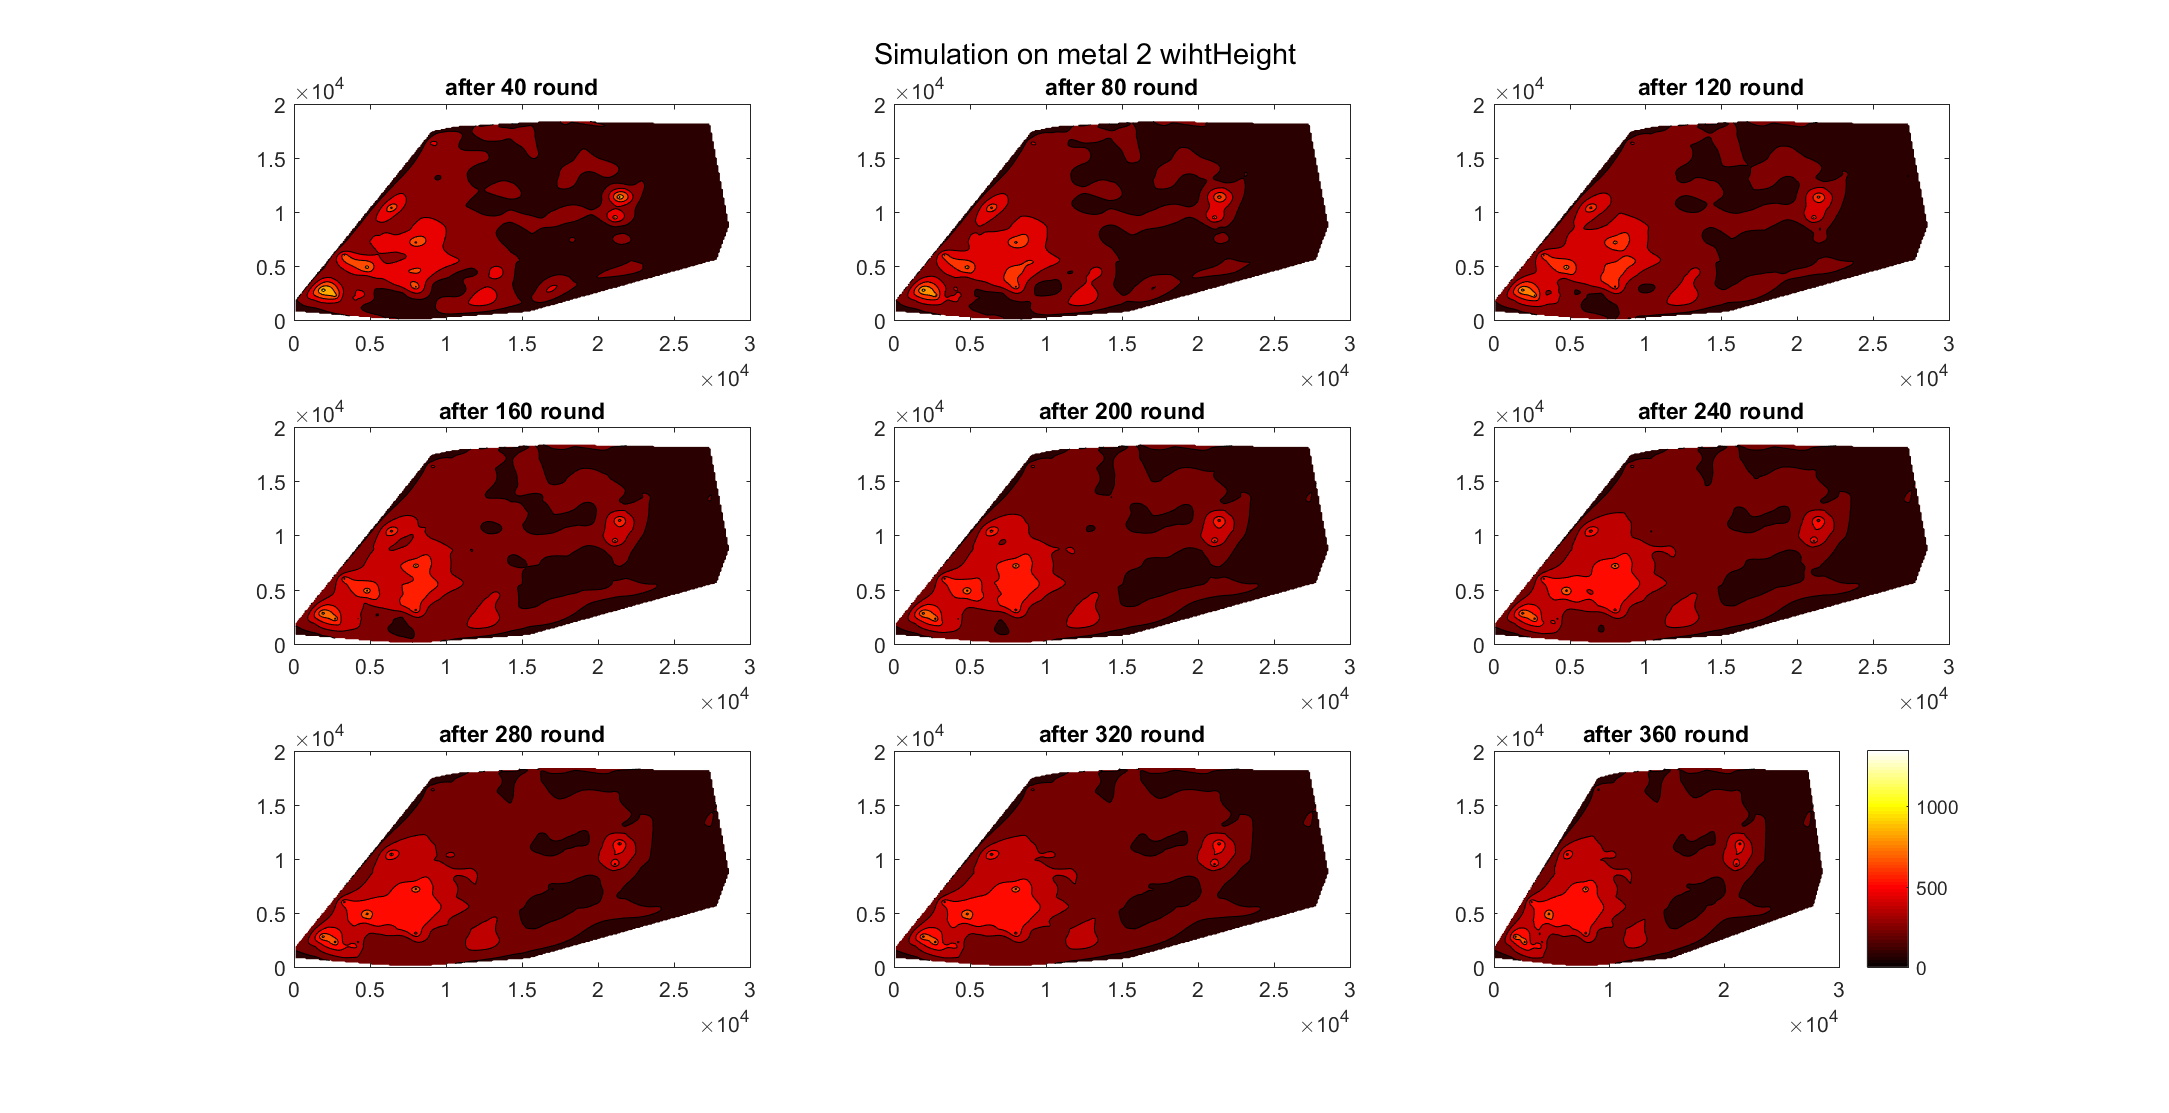
\includegraphics[scale=0.5]{pictures/pollution-with-hight-Cd.eps}
    \caption{城市土壤变化情况}
    \label{fig:pollution-with-hight}
\end{figure}
可以看出
\subsection{三种模型的结果比较}
分别分析了以上三种模型,接下来我们来考察一下经过一段时间后,三种不同方案对于城市土壤变化的不同影响。
并从中分析土壤治理中应该注意的问题。\\
\indent 我们依然使用Cd作为模拟的重金属元素。我们将经过的时间设为一年。
即比较采取不同的方案一年之后,城市土壤重金属的含量。经过MATLAB模拟后,我们得到图\ref{fig:different-model-comparison-of-Cd}。
\begin{figure}
    %\centering 
    \flushleft
    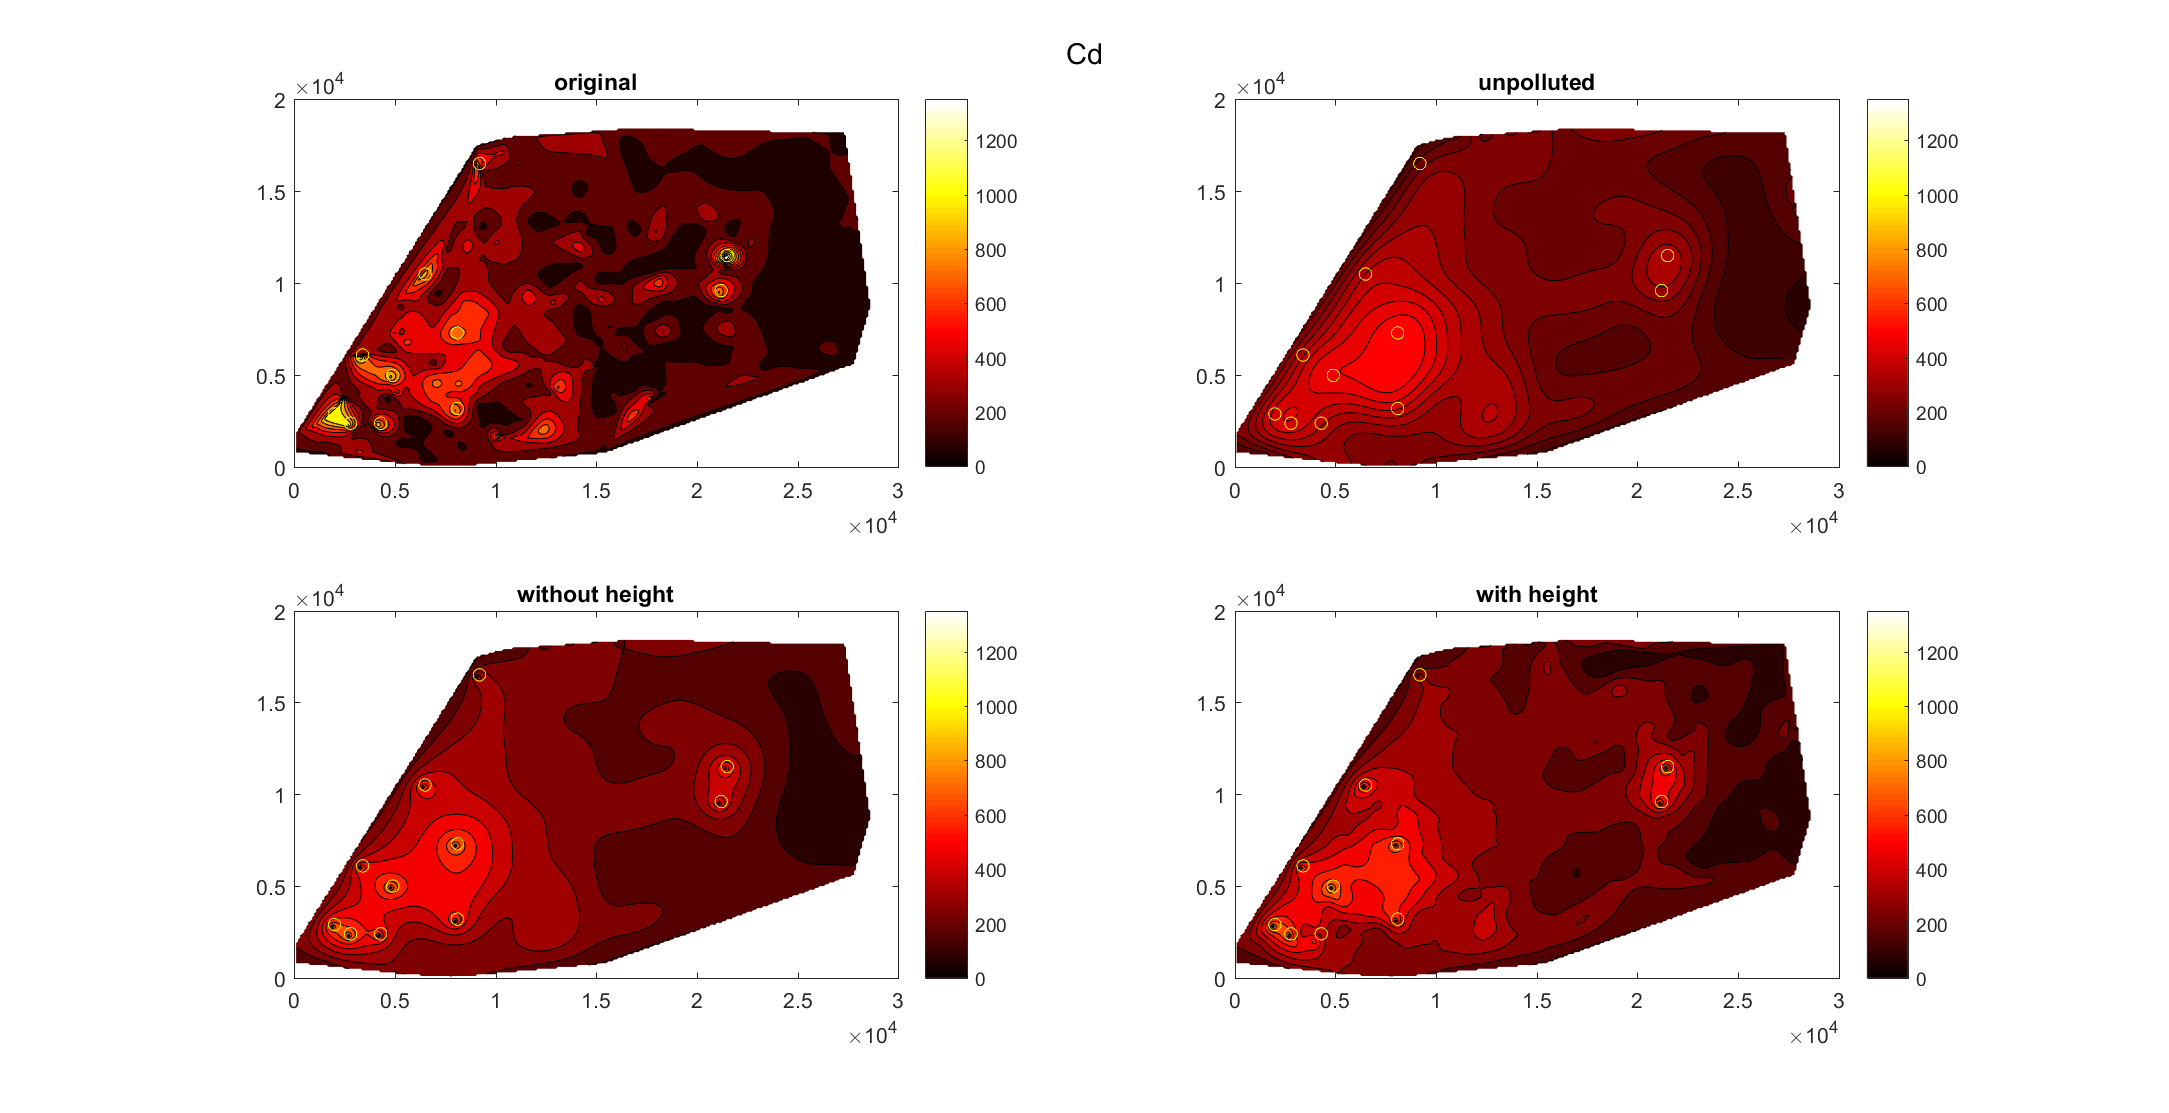
\includegraphics[scale=0.5]{pictures/different-model-comparison-of-Cd.eps}
    \caption{不同方案的比较}
    \label{fig:different-model-comparison-of-Cd}
\end{figure}
注意图中的深色区域表示重金属含量低的地区,而颜色较浅的区域表示重金属含量高的地区。
通过图像的对比,我们可以清楚地看出
\begin{itemize}
\item 在杜绝所有的污染源排放重金属污染物之后,重金属污染物含量的峰值相比于其他两种方案大大减少。
这说明大力从源头上减少重金属污染的排放对于重金属污染的治理是十分有效的。
我们应该倡导企业做到污水处理后再排放,以减少排放到环境中的重金属的含量
\item 但从三种方案均可以看出,之前已经受到污染的地区仍会向周围不断地传播,污染那些重金属含量低的地区。
这说明我们在治理重金属污染物时,不能仅仅只是减少污染物的排放,还要考虑已经产生的重金属污染物的降解问题。
这样才可以防止重金属污染严重地区对于周围未被污染的土壤的影响。
\item 通过对比左边的两张图,我们可以看出,经过一年的时间,该城区的土壤重金属含量与之前有了很大的改变,城区的土壤重金属含量有大范围的增长。
这告诉我们,对于那些高重金属污染的工厂,我们应该坚决关停,否则城市的土壤重金属含量就会向我们所模拟的那样,
在短短几年之内,对城市的土壤造成大范围的污染,严重影响城市居民的生活健康
\item 再对比下面的两张图,这显示了考虑城市的地势与否对模拟结果造成的影响。
通过比较,尽管我们假设的由地势造成的扩散系数很小,但经过一段时间的积累,它对于城市土壤重金属含量的分布依然造成了很大的影响。
对比这两张图的左下角,同时参看该城区的地形分布图,可以看出由于地形的原因,
两个比较接近的污染源之间的地区的地势低于两个污染源,从而重金属污染物向中间区域传播速率很快,
从而导致中间地带的重金属污染程度与污染源的重金属污染程度基本相同。
这也给了我们一个启示:工厂如果建在地势较低的地区,那么其排放的重金属污染向周围的传播速度就会因为地势的原因而减慢。
这样就会减慢土壤污染面积的扩大。
\end{itemize}
\part{模型的完善}
在实际的土壤环境中,由于空气氧化,土壤中发生的化学发应以及微生物对于重金属污染的降解作用,土壤在一定的重金属污染范围内是具有自我净化功能的。
所以作为模型的完善,我们可以考虑土壤的重金属降解速率$\gamma$。从而得到重金属的降解模型
土壤中重金属的来源是多途径的,首先是成土母质本身含有重金属,不同的母质、成土过程所形成的土壤含有重金属量差异很大。
此外,人类工农业生产活动,也造成重金属对大气、水体和土壤的污染,而大气和水体中的重金属又会反过来对土壤的污染造成影响。
在前面的建模过程中,我们仅仅只考虑了土壤和地势对于重金属传播的影响,而没有考虑水体以及空气的因素。
\section{重金属降解模型}
在这一节中,我们考察重金属在土壤中的降解对于模型的修正。
这一部分的背景资料我们参考了 \cite{art:jiangjie} 。
由于重金属的降解是一个非常缓慢的过程,因此这个修正造成的影响是不显著的。
亦即,在重点被污染的地区,降解的速度是远远跟不上排放速度的;
但是,在生活区、公园区等污染程度较轻的区域,降解还是有可能能够减缓当地被污染的情况。

考虑在单位时间内,单位区域内由于某种降解机制引起了该地区重金属浓度的减少量 $\Delta_d \rho$ :
\begin{itemize}
	\item 当重金属浓度很低的时候,能够完全降解;
	\item 当重金属浓度超过某一水平 $f_1$ 时,不能完全降解,但是减少的量随着金属浓度的增加而增加,即
		$$ \Delta_d \rho = f_1 + \gamma (\rho - f_1) $$
	\item 当重金属浓度超过另一水平 $f_2$ ,降解机制已经达到饱和,不能降解剩余的重金属,于是
		$$ \Delta_d \rho = f_1 + \gamma (f_2 - f_1) $$
\end{itemize}
于是,我们将式 \eqref{eqn_model} 修正为
$$ \frac{\partial \rho}{\partial t} = \kappa \Delta \rho + \tau \Delta h \cdot \rho - \Delta_d \rho $$
这里
\[
	\Delta_d \rho = 
	\begin{cases}
		\rho & 0 \le \rho < f_1 \\
		f_1 + \gamma (\rho - f_1) & f_1 \le \rho < f_2 \\
		f_1 + \gamma (f_2 - f_1) & f_2 \le \rho
	\end{cases}
\]

为了模拟上述方程所对应模型的发展趋势,我们需要收集不同重金属所对应的降解原理,以及对应的降解速度 $\gamma$ 。

\section{重金属水体传播模型}
这里首先要明确,我们所关注的水体并非完全“清澈”的纯净水体,而是在一般城市中较为常见的含泥沙的复杂水体。
在这种水体中,起主导作用的重金属依存方式是吸附在泥沙上而不是仅仅溶解在水溶液中,因此我们研究的重点是含泥沙的悬浊液中重金属浓度的传播模式。
参考 \cite{hsl:515} 对于水中重金属浓度的分析,我们可以建立起重金属的水体传播模型。
\subsection{一些假定}
为了简化模型的复杂程度,我们做出如下假设:
\begin{itemize}
	\item 在整个水深范围内, 浓度分布由三部分组成:上部是悬移质泥沙和水流运动空间,中间部分是推移质泥沙和水流运动空间,下部是河床冲淤变形的区域。
	\item 河床变形区域内孔隙水相对整个断面也较小,因此忽略其中的重金属,同时忽略生物化学作用传质,不考虑生物体对重金属的富集。
	\item 在河流的宽度方向上重金属浓度保持不变;这是考虑到我们关注的浓度变化存在于河流的流动方向上(一般长度在 $10^3$ 米左右),而相比于此河流的宽度(一般在 $10^1$ 米左右)可以忽略不计,因此浓度在宽度方向上是相同的。
	\item 对于颗粒相浓度的变化(悬浮质颗粒相、推移质颗粒相和床沙质颗粒相重金属污染物浓度),吸附-解吸是其生物-化学反应的主要机理。
\end{itemize}
\subsection{记号表}
\begin{table}[H]
	\centering
	\caption{关于重金属水体传播模型的记号说明}
	\label{tab:water_model_symbols}
	\begin{tabular}{cc}
		\hline
		符号 & 含义  \\
		\hline
		$l$ & 沿河流的长度参数   \\
		$H$ & 河流的宽度  \\
		$c$ & 溶解相重金属污染物垂线(水深)平均浓度  \\
		$u$ & 沿河流方向水流和悬移质泥沙垂线平均流速 \\
		$w_l$ & 沿河流方向推移质泥沙和水流垂线平均流速      \\
		$s_x$ & 垂线平均的悬移质(s)和推移质(b)泥沙浓度      \\
		$N_s$ & 垂线平均的悬移质泥沙颗粒相(悬浮颗粒相)重金属污染物浓度 \\
		$N_b$ & 推移质泥沙颗粒相(推移颗粒相)重金属污染物浓度 \\
		$N_m$ & 床沙质泥沙颗粒相(床沙颗粒相)重金属污染物浓度 \\
		$h_1$ & 悬移质泥沙(水流)占据的水深 \\
		$h_2$ & 推移质泥沙(水流)占据的水深 \\
		$h_3$ & 河床变形的深度 \\
		$h$ & 水深 $(=h_1+h_2)$ \\
		$\rho_s$ & 泥沙颗粒的比重 \\
		$p^{'}$ & 河床的孔隙度 \\
		\hline	
	\end{tabular} \\
\end{table}
\subsection{方程的建立}
考虑在在 $dt$ 时间内, $dl$ 长的一段内重金属的变化量:
\[ \begin{split}
&\frac{\partial}{\partial t}\left[c\left(h_1\left(1-\frac{s_s}{\rho_s}\right) + h_2\left(1-\frac{s_b}{\rho_s}\right)\right)Hdl\right]dt \\
+ &\frac{\partial}{\partial t}(s_sN_sh_1Hdl)dt \\
+ &\frac{\partial}{\partial t}(s_bN_bh_2Hdl)dt \\
+ &\frac{\partial}{\partial t}(N_m(1-p^{'})Hdl)dt 
\end{split} \]
最后一项是床沙质泥沙上重金属量的变化。

同时考虑在 $dt$ 时间内,因为水的流动而造成的河流 $dl$ 长的一段内水相、悬浮颗粒相、推移颗粒相的增加量:
\begin{itemize}
	\item 水相
		$$ -\frac{\partial}{\partial l}\left[uh_1cH\left(1-\frac{s_s}{\rho_s}\right)\right]dldt -\frac{\partial}{\partial l}\left[w_lh_2cH\left(1-\frac{s_b}{\rho_s}\right)\right]dldt $$
	\item 悬浮颗粒相
		$$ -\frac{\partial}{\partial l}(us_sN_sh_1H)dldt $$
	\item 推移颗粒相
		$$ -\frac{\partial}{\partial l}(w_ls_bN_bh_2H)dldt $$
\end{itemize}

由于质量守恒,上述的两组效应应该达到精确的平衡。
考虑在大多数冲积河流中,推移质泥沙运动一般较小,可以忽略。
此时有 $h_2 = 0$ 和 $h = h_1$;因此化简得到
$$ \frac{\partial c}{\partial t} + u\frac{\partial c}{\partial l} + \frac{1}{h} \frac{\partial}{\partial l}\left(h E_l \frac{\partial c}{\partial l}\right) = N_s \frac{\rho^{'}}{h} \frac{\partial h_3}{\partial t} - \frac{1 - p^{'}}{h}\frac{\partial N_m}{\partial t} - \left[ s_s\frac{\partial N_s}{\partial t} + s_s u \frac{\partial N_s}{\partial l} -E_l^s\frac{\partial s_s}{\partial l}\frac{\partial N_s}{\partial l} \right]$$

\subsection{模型的定性分析}
这个模型已经能够解决在给定污染分布情况下,计算重金属浓度分布随时间的变化趋势。
然而,同上面的论述一样,我们更为关心的问题是,在改变污染源排放力度的情况下,河流重金属污染程度会发生什么变化。

基于我们已有的数据,如果能够结合当地水流的地形图,我们可以通过取最邻近水域的方式将重点排污区“移动”到河流上。
那么在这种近似下,我们只需要确定这个次级模型中关于泥沙流动速度、泥沙浓度、泥沙吸附重金属离子速度等参数。

可以预见到的是,如果在完全没有排污的情况下,由于水流流动的作用,重金属的浓度将会随时间逐渐降低,而且从水流的上游逐渐向下游传递。
但是在工厂等外在排放因素的干扰下,随着排污速度的增加,可能在突破某个临界点之后会使得某一段的水域呈现出持续的污染。
因此治理方案可以是将大工厂拆散成几个小工厂,以符合泥沙的吸收速率,从而降低重金属离子在水中的溶解浓度,达到减少污染危害的目的。

\section{重金属空气传播模型}
重金属在空气中传播的模型和在土壤、水流中传播的模型有很大的差异。
这是因为在空气中,对流速度比起在水流中要大得多,因此由空气携带的污染通过流动的方式进行传播,而不是像土壤模型那样是通过扩散进行的。
于是,我们需要参考其他的理论 \cite{air_model} 来建立精细的模型。

考虑在式 \eqref{eqn_model} 的推导过程中,我们假定土壤是不会发生流动的;但是这个假定在空气中是完全不能成立的。
尽管如此,空气传播模型仍然在一定程度上能够遵守热传播模型,只是我们需要对于空气能够流动这个“例外”加以修正。

考虑单位体积的空气,正以 $\textbf{v}$ 的速度运动,那么污染浓度的增加量有两部分组成:一部分是由于扩散到两边空气的扩散差,另一部分是空气的自然流动而造成有浓度差异的空气流动到这个位置引起的浓度差。
因此,我们需要加以修正的恰是后面这一项,得到
$$ \frac{\partial \rho}{\partial t} + \nabla(\textbf{v} \cdot \rho) = \kappa \Delta \rho + \tau \Delta h \cdot \rho - \Delta_d  $$
这里 $\Delta_d$ 指空气中重金属的降解速度。


\part{对于该城区环境治理的建议}
在改革开放的几十年里,我国的在经济上取得了飞速的发展,但在很大程度上是以牺牲环境为代价得到的。
到现在,可以说环境问题已经非常严重,治理环境污染刻不容缓。而土壤污染的治理也是环境治理的重点。
这是因为土壤环境状况直接影响老百姓的菜篮子、米袋子,更是国土资源环境安全和经济社会可持续发展的重要因素。
可以说没有一个良好的土壤环境,国家的发展繁荣就无从谈起。  \\
\indent 而就现实而言,目前的土壤重金属污染形势十分严峻,有些地区的土壤污染及其严重,对当地居民的生活健康都造成巨大的影响。
就如本文中的城区,由第一问的结果可以看出,大部分区域都处于中等污染的程度,而工业区则是污染非常严重,这严重危害了城区的形象和居民的身体健康。
对于该城区,如果置之不理,由我们的分析可看出,该城区的土壤环境将会变得更加恶劣。  \\
\indent 为此,我们给该城区的相关部门提出以下意见:
\begin{itemize}
\item 从功能分区图上可以看出,部分工业区和生活区距离过近,甚至有产生共同区
域的情况,这对人们的日常生活和身体健康都是有害的,故建议把工厂全部迁到城区的
下风带,或是将生活区全部迁至城区的上风带且远离工业区的地方。
\item 由第三部分的分析结果我们知道,绿化带有抑制重金属元素富集或传播的作用,故建
议大力开展植树造林。不仅美化了城区形象,还可以平衡重金属污染物的破坏效应。
\item 由于该城区交通污染较为严重,建议推广电瓶车的使用或倡导居民出行时步
行或自行车,尽量减少汽车尾气的排放。
\item 该城区的燃煤污染也较为严重,建议大力推广天然气或者石油气的使用。
\item 该城区也存在矿区污染的问题,建议当地政府应做好环境保护措施,并加大检
查力度,确保矿区的酸性废水达到可以排放的标准之后再排放。
\item 由第四部分的分析可知,对于那些有高重金属污染排放量的工厂,我们应该坚决责令其整改或关停绝对不能姑息。
否则这些高污染工厂对于周围的环境将会造成十分严重的危害。
\item 此外政府也应该着力去寻找重金属降解的新方法,尽力去把那些已经遭到严重污染的土壤中的有毒重金属成分通过物理化学生物方法转化为毒性较弱或者无毒的物质,
从而达到土质净化的目的,同时也避免严重污染的土壤对于未污染土壤的影响。
\item 此外还建议把工厂尽量搬迁到地势较低的地区。这样可以有效的降低重金属污染的传播速率,从而减少重金属污染地区的面积。
\end{itemize}
\indent 土地孕育了我们人类的文明,我们也应该尽力的去保护我们赖以生存的土地。
不要为了今日的一时之利而破坏了它。希望相关部门能够早日真正的行动起来,担起保护土壤的重任,为我们的未来出一份力。







% part 3
% 局部污染源的寻找
% 
% 对于污染传播建模
% 
% 模拟,使用不同的治理策略
% - 完全关停(+高度项)
% - 放任(+高度项)
% 注:高度项是修正
% 涉及到具体浓度的计算
% 
% part4
% 
% - 土壤,水,空气模型(分离)
% 
% - 重金属降解模型
% 
% - 建议




\printbibliography
\end{document}